\documentclass[conference]{IEEEtran}
\IEEEoverridecommandlockouts
\usepackage{fontspec}   % Times text as in the IEEE sample (Tectonic/XeTeX has no Type-1 Times)
\setmainfont{Times New Roman}
\setmonofont{Courier New}[Scale=0.9]
\usepackage{cite}
\usepackage{amsmath}
\usepackage{graphicx}
\usepackage{booktabs}
\usepackage{algorithm}
\usepackage{algorithmic}
\usepackage{multirow}
\usepackage{array}
\usepackage{xcolor}
\usepackage{url}
\usepackage{xurl}
\usepackage{hyperref}
\hypersetup{colorlinks=true, linkcolor=black, citecolor=black, urlcolor=blue}
\def\BibTeX{{\rm B\kern-.05em{\sc i\kern-.025em b}\kern-.08em T\kern-.1667em\lower.7ex\hbox{E}\kern-.125em X}}

\begin{document}

\title{QueryGenie: Confidence-Aware Abstention for\\Open-Weight Text-to-SQL}

\author{\IEEEauthorblockN{1\textsuperscript{st} N V V S S Jayakanth Kamisetti}
\IEEEauthorblockA{\textit{Dept. of Computer Science and IT} \\
\textit{KL University}\\
Hyderabad, India \\
2320090050}
\and
\IEEEauthorblockN{2\textsuperscript{nd} Boddupally Narendar}
\IEEEauthorblockA{\textit{Dept. of Computer Science and IT} \\
\textit{KL University}\\
Hyderabad, India \\
2320090009}
\and
\IEEEauthorblockN{3\textsuperscript{rd} M Praneeth Reddy}
\IEEEauthorblockA{\textit{Dept. of Computer Science and IT} \\
\textit{KL University}\\
Hyderabad, India \\
2320090018}
\and
\IEEEauthorblockN{Supervisor: M Parameswar}
\IEEEauthorblockA{\textit{Associate Professor, Dept. of Computer Science and IT} \\
\textit{KL University}\\
Hyderabad, India}}

\maketitle

\begin{abstract}
Open-weight text-to-SQL models such as CodeS return one query per question and give no indication of whether it can be trusted. We reproduce the open CodeS-1B model, then make it say when it is unsure. On the 1,034 Spider development questions we measure 77.8\% execution accuracy against the paper's 77.9\%, using the authors' own evaluator. We execute the four candidate queries that beam search already produces, count how many return the same result, and abstain when that agreement is low. At 90.4\% coverage the system is right 83.3\% of the time instead of 77.8\%, and gives 156 wrong answers instead of 230; over ten calibration/test splits the gain over random abstention is $+5.46$ points (paired $t$-test $p=7.7\times10^{-10}$, Wilcoxon $p=9.8\times10^{-4}$, bootstrap 95\% CI $[+4.5,+6.7]$). Because beam candidates are often copies, we measure how many are different (all four in 56\% of questions) and repeat the study over different queries only, with CodeS-3B, and with eight sampled candidates; the gain holds in each. The pipeline reaches 69.5\% on Spider-Realistic (paper: 70.9\%) and runs on a live PostgreSQL database through a read-only SQL translation, where 94.4\% of the Spider gold queries return the same rows as on SQLite. It ships as a desktop application that runs locally; code and logs are at github.com/jayakanthh/QueryGenie. Test-suite accuracy and a full BIRD evaluation are TBD.
\end{abstract}

\begin{IEEEkeywords}
text-to-SQL, selective prediction, abstention, execution agreement, reproducibility, CodeS, Spider
\end{IEEEkeywords}

\section{Introduction}
A natural-language interface to a database is only useful if its users can tell when to believe it. Text-to-SQL models are usually compared by how often they are right when they answer every question \cite{deng2022recent, hong2024nextgeneration}, but a wrong query is more costly than no query: it returns a plausible table that looks like an answer. Many high-scoring systems rely on closed hosted models \cite{pourreza2023dinsql, gao2023texttosql, pourreza2024chasesql}, which means a company's schema is sent to a third party. CodeS \cite{li2024codes} offers open models of 1B to 15B parameters that score as well on Spider, but it returns one query per question with uniform apparent confidence. Confidence estimation and abstention for semantic parsing and text-to-SQL have been studied \cite{stengel2023calibrated, somov2025confidence, lee2024trustsql, maleki2025confidence}, including consistency over candidates and execution results \cite{maleki2025confidence, borchmann2025query}; we do not claim execution agreement as a new idea. Our contribution is to measure it carefully on a reproduced open model and to put it into a working local application.

This paper does three things.
\begin{enumerate}
\item \textbf{Reproduction.} We reproduce SFT CodeS-1B on Spider \cite{yu2018spider} within 0.2 points of the published figure (77.76\% against 77.9\%), after auditing our harness line by line against the authors' code and fixing the errors that audit found (Section~\ref{sec:repro}).
\item \textbf{Confidence-aware abstention.} We use the candidates CodeS already generates (no extra model or training): the system executes all of them, measures how many agree on a result, and declines to answer, with a clarifying choice, when agreement is low. We evaluate this as an accuracy--coverage trade-off with a pre-registered significance protocol (Section~\ref{sec:abstain}).
\item \textbf{Candidate diversity and other settings.} We test the claim behind the method --- that agreement among candidates carries information --- when the candidates are partly duplicates, with a larger model, with sampled candidates, on rewritten questions and on a live PostgreSQL server (Sections~\ref{sec:diversity}--\ref{sec:beyond}).
\end{enumerate}

All numbers below come from logged runs (seed 42, hardware and runtime recorded for each) and the scripts that analyse them; a number we did not measure is marked TBD. The code, run logs and analysis scripts are in the project repository, \url{https://github.com/jayakanthh/QueryGenie}.

\section{Related Work}
Spider \cite{yu2018spider} is the standard cross-domain benchmark, scored today by execution rather than by string match, with test-suite accuracy \cite{zhong2020semantic} as a stricter variant. Spider-Realistic \cite{deng2020structuregrounded}, Spider-Syn \cite{gan2021towards} and BIRD \cite{li2023can} probe robustness to wording, synonyms and large real-world databases. Methods moved from graph encoders \cite{wang2019ratsql, cao2021lgesql} and constrained decoding \cite{scholak2021picard} to large language models, prompted \cite{pourreza2023dinsql, gao2023texttosql, wang2023macsql, talaei2024chess} or fine-tuned \cite{li2024codes, li2023resdsql}. Value matching in the style of BRIDGE \cite{lin2020bridging}, which CodeS keeps, adds matched cell values to the prompt.

\textbf{Confidence and abstention.} Our rule combines two older ideas: self-consistency, which trusts the answer that most sampled reasoning paths reach \cite{wang2022selfconsistency}, and selective classification, which lets a model decline inputs and reports the accuracy--coverage trade-off \cite{geifman2017selective}. For semantic parsing, Stengel-Eskin and Van Durme study confidence estimation \cite{stengel2023calibrated} and, in ``Did You Mean...?'', use calibrated confidence to decide when to ask the user for help, trading safety against convenience \cite{stengel2023did}, the same trade-off our application faces. For text-to-SQL, Somov and Tutubalina \cite{somov2025confidence} add selective classifiers and study entropy-based confidence and its coverage--risk trade-off; Maleki et al.\ \cite{maleki2025confidence} compare black-box and white-box confidence estimates for generated SQL and find consistency-based methods the strongest black-box choice, with execution adding signal; Liu et al.\ \cite{liu2025calibrating} calibrate confidence from sub-clause frequencies over several samples; TrustSQL \cite{lee2024trustsql} and EHRSQL \cite{lee2022ehrsql} score systems on answering feasible questions and abstaining on infeasible ones; and Chen et al.\ \cite{chen2025reliable} abstain at the schema-linking step. Execution results have also been used to rerank candidate programs \cite{ni2023lever}, to pick the most execution-consistent query \cite{borchmann2025query}, and in DAIL-SQL's voting \cite{gao2023texttosql}. Recent studies compare confidence signals for generated SQL \cite{richardson2026predicts} and show that the risk a conformal abstention rule reports depends on the execution oracle that labels correctness \cite{liu2026certified}. Questions with several valid queries are the subject of AmbiQT \cite{bhaskar2023benchmarking} and AMBROSIA \cite{saparina2024ambrosia}, which is the situation in which our application shows the competing readings. Against this background our contribution is narrower: a reproduced open 1B model, agreement over the candidates it already produces, a pre-registered significance protocol, a check of the signal against duplicated candidates and other settings, and an application that offers the user the competing readings when it abstains.

\textbf{Repair.} Execution-guided repair, in the spirit of DIN-SQL's self-correction \cite{pourreza2023dinsql}, addresses queries that fail; we measure it and find that it addresses a small share of CodeS's errors (Section~\ref{sec:abstain}).

\section{Experimental Setup and Reproduction}
\label{sec:repro}
\textbf{Data.} All data come from approved public sources on Hugging Face (Table~\ref{tab:setup}). Spider's development databases are small (2 to 11 tables, 7 to 56 columns) and its questions often name the columns; 39.5\% of the gold queries need a join, 26.8\% a \texttt{GROUP BY}, 8.0\% a nested query and 7.7\% a set operation. By the official difficulty classifier the 1,034 questions are 248 easy, 446 medium, 174 hard and 166 extra hard.

\begin{table}[t]
\centering
\caption{Evaluation sets and setup. All runs use seed 42.}
\label{tab:setup}
\small\setlength{\tabcolsep}{3pt}
\begin{tabular}{@{}lp{5.2cm}@{}}
\toprule
Spider dev & 1,034 questions, 20 databases (reproduction, ablation, abstention) \\
Spider-Realistic & 508 questions, 19 databases (rewritten wording) \\
BIRD Mini-Dev & 500 questions, 11 databases (stopped, not reported) \\
Metric & official Spider execution match (\texttt{evaluation.py --etype exec}) \\
Decoding & 4 beams, at most 256 new tokens, prompts cut to 3,840 tokens \\
Hardware & Colab Tesla T4, fp16 (CodeS-1B, 3B, sampling); Apple M4, bf16 (Spider-Realistic, application) \\
Software & PyTorch 2.11 and transformers 5.16 (T4); PyTorch 2.13 and transformers 5.15 (M4) \\
Run time & 2,865 s for one Spider dev pass of CodeS-1B (T4); 5,543 s for CodeS-3B \\
\bottomrule
\end{tabular}
\end{table}

\textbf{Pipeline.} For each question CodeS builds a prompt from the database: every table with its columns, types, keys and representative values, human-readable column descriptions, and stored values matched to words in the question by the authors' value retriever. The model generates four candidates by beam search and returns the first that SQLite accepts (\texttt{EXPLAIN QUERY PLAN}), otherwise the first beam. We use the authors' fine-tuned \texttt{seeklhy/codes-1b-spider} (and \texttt{codes-3b-spider}), fp16.

\textbf{Harness audit.} Our first runs scored 64.8--73.8\%. We compared the harness line by line with the authors' code and found a bug in our port (numbers were never matched by the value retriever, changing the prompt for 12.4\% of questions), missing column descriptions, and a simplified scoring metric that was not the paper's. We fixed these, switched to the official evaluator \cite{zhong2020semantic} (execution match), and kept the earlier runs in the log, marked as superseded.

\textbf{Result.} The corrected pipeline reaches 77.8\% execution accuracy (804/1034; run T2-005, re-run from scratch as T2-006 with an identical result), against 77.9\% in the paper. Table~\ref{tab:repro} shows the effect of each fix and of the model size. The 3B model reaches 81.8\% (paper: 83.4\%, $-1.6$ points). The paper also reports test-suite accuracy of 72.2\% for CodeS-1B; we did not compute ours (TBD).

\begin{table}[t]
\centering
\caption{Execution accuracy (EX) on Spider dev, 1,034 questions.}
\label{tab:repro}
\small
\begin{tabular}{@{}llr@{}}
\toprule
Run & Setting & EX \\
\midrule
T2-001 & no value retriever, simple metric & 64.8\% \\
T2-003 & full prompt, simple metric & 73.8\% \\
\textbf{T2-005} & \textbf{audited harness, official metric} & \textbf{77.8\%} \\
 & \emph{paper, CodeS-1B} & \emph{77.9\%} \\
T2-004 & CodeS-3B, official metric & 81.8\% \\
 & \emph{paper, CodeS-3B} & \emph{83.4\%} \\
\bottomrule
\end{tabular}
\end{table}

\textbf{Ablation.} Removing one component at a time (official metric, same model and seed) lowers accuracy in every case (Table~\ref{tab:ablation}). The differences are 9--20 questions each and were not tested for significance, so the order of the two smallest effects should not be over-read. Accuracy falls with difficulty: 90.3\% on easy, 83.6\% medium, 64.9\% hard and 56.6\% extra-hard questions.

\begin{table}[t]
\centering
\caption{Ablation on Spider dev (CodeS-1B, official metric).}
\label{tab:ablation}
\small
\begin{tabular}{@{}llrrr@{}}
\toprule
Run & Component removed & EX & $\Delta$ & Executable \\
\midrule
T2-005 & none (full pipeline) & 77.8\% & --- & 97.3\% \\
AB-105 & foreign keys & 76.9\% & $-0.9$ & 95.9\% \\
AB-103 & column values & 76.4\% & $-1.4$ & 98.1\% \\
AB-106 & selection (beam 0 only) & 76.0\% & $-1.8$ & 94.1\% \\
AB-104 & value retriever & 75.9\% & $-1.9$ & 97.2\% \\
\bottomrule
\end{tabular}
\end{table}

\textbf{Deviations.} We match values by scanning all distinct values rather than the authors' Lucene BM25 pre-filter; we do not apply the optional schema classifier; and we use newer PyTorch and transformers versions on one T4 instead of eight A800 GPUs.

\section{Confidence-Aware Abstention}
\label{sec:abstain}
\begin{figure*}[t]
\centering
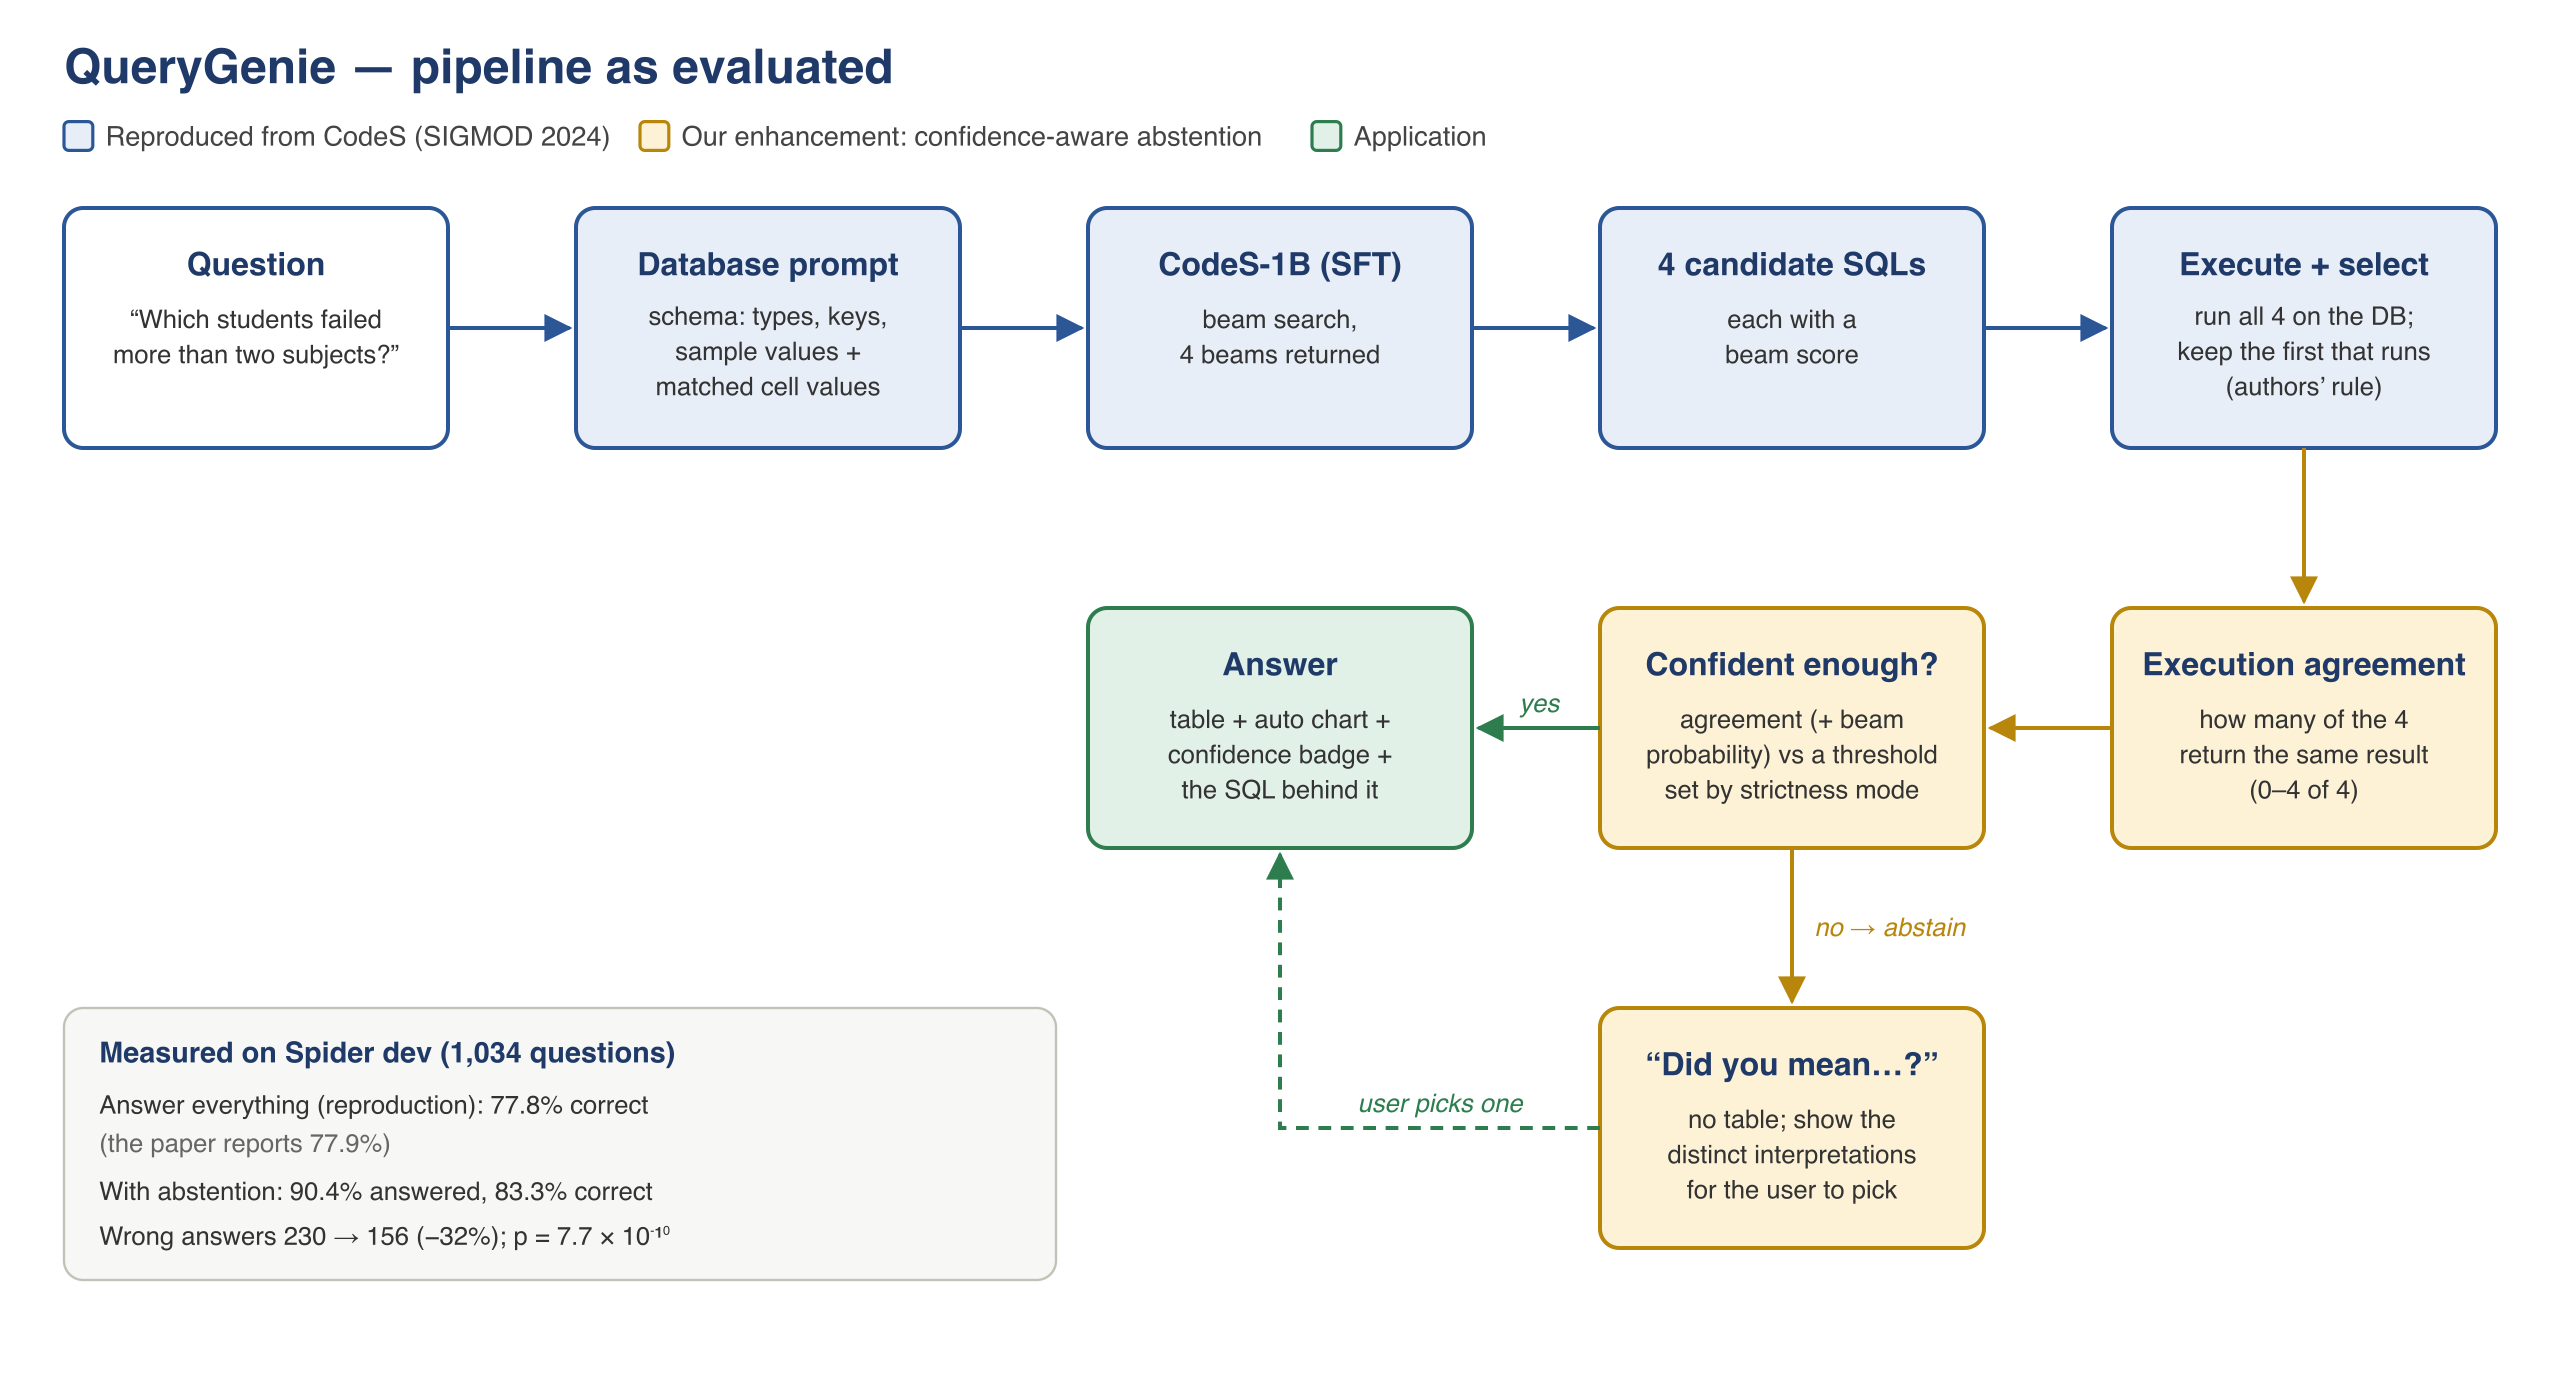
\includegraphics[width=0.8\textwidth]{figures/final_pipeline.png}
\caption{System architecture: the reproduced CodeS components, the abstention step added here, and the application.}
\label{fig:pipeline}
\end{figure*}

\textbf{Method.} Of the 97.3\% of queries that execute, many still return the wrong rows, so repairing failures cannot fix most errors. Execution-guided repair, which returns each failed query to the model once together with its error message, was tried on 377 failed queries over 211 questions; 61 then ran and one more answer became correct (77.76\% $\to$ 77.85\%). We therefore turned to the queries that run but are wrong. All candidates are executed (read-only, on the original database); the \emph{agreement} $a$ of the returned answer is the share of candidates whose result equals it, and $0$ if the returned query fails. The confidence is $c=a+0.01\,p_b$, where $p_b$ is the softmax beam probability of the returned candidate (a tie-breaker only). The system abstains when $c<\tau$: it then shows no table, but lists the distinct results of the candidates as readings for the user to choose from (Algorithm~\ref{alg:abstain}, Fig.~\ref{fig:pipeline}). No model is retrained.

\begin{algorithm}[t]
\caption{Answer or ask, for one question}
\label{alg:abstain}
\begin{algorithmic}[1]
\small
\REQUIRE question $Q$, database $D$, threshold $\tau$
\STATE $P \leftarrow$ CodeS database prompt for $(Q,D)$
\STATE $(s_1,\dots,s_4),(b_1,\dots,b_4) \leftarrow$ four beam candidates and scores
\FOR{$i=1$ \TO $4$}
  \STATE $r_i \leftarrow$ result of running $s_i$ on $D$ (read-only; none if it fails)
\ENDFOR
\STATE $k \leftarrow$ first $i$ whose query passes \texttt{EXPLAIN QUERY PLAN}, else $1$
\STATE $a \leftarrow \tfrac14\lvert\{i: r_i = r_k\}\rvert$ if $s_k$ runs, else $0$
\STATE $c \leftarrow a + 0.01\,e^{b_k}/\sum_j e^{b_j}$
\IF{$c \ge \tau$}
  \RETURN result $r_k$ and agreement $a$
\ELSE
  \RETURN the distinct results among $r_1,\dots,r_4$ as readings to choose from
\ENDIF
\end{algorithmic}
\end{algorithm}

\textbf{Protocol.} Fixed before the results were seen: ten random 50/50 calibration/test splits of the 1,034 questions; $\tau$ chosen on the calibration half for at least 90\% coverage and applied to the test half; accuracy on answered questions compared with random abstention at the same coverage (the model's accuracy on that half); one-sided paired $t$-test and Wilcoxon signed-rank test at $\alpha=0.05$; and a question-level bootstrap (5,000 resamples) that does not rely on the splits being independent. The protocol was written in the Week-9 enhancement proposal. The deployed threshold, $\tau=0.2526$, is the median over the ten calibration halves. In words: abstain when no candidate runs, or when only one of four supports the answer and its beam probability is below about 0.26.

\textbf{Results.} Table~\ref{tab:abstain} and Fig.~\ref{fig:curve} show the outcome. At 90.4\% coverage the system answers correctly 83.3\% of the time against 77.8\% for answering everything (this full-set figure applies the deployed $\tau$ to the questions it was calibrated on; the held-out mean over the ten splits is 83.25\% at 90.5\% coverage); wrong answers fall from 230 to 156 ($-32\%$). Of the 99 questions it declines, 74 would have been wrong and 25 correct. The mean gain over random abstention is $+5.46$ points (SD 0.71), positive in all ten splits: paired $t=24.4$, $p=7.7\times10^{-10}$; Wilcoxon $W=55$, $p=9.8\times10^{-4}$ (the smallest value possible with ten pairs); bootstrap 95\% CI $[+4.51,+6.71]$. We reject the null hypothesis of no gain. Beam probability alone gives a smaller gain ($+3.08$ points); agreement is higher than beam probability by 2.37 points on the same splits (paired $t=6.31$, $p=1.4\times10^{-4}$).

\begin{table}[t]
\centering
\caption{Answering everything vs.\ abstaining (CodeS-1B, run T2-006).}
\label{tab:abstain}
\small\setlength{\tabcolsep}{3pt}
\begin{tabular}{@{}lrrr@{}}
\toprule
Setting & Answered & Acc.\ on answered & Wrong \\
\midrule
Answer everything & 1,034 (100\%) & 77.76\% & 230 \\
\textbf{Balanced ($\tau=0.2526$)} & \textbf{935 (90.4\%)} & \textbf{83.32\%} & \textbf{156} \\
Strict ($\ge$3 of 4 agree) & 649 (62.8\%) & 86.13\% & 90 \\
Very strict (all 4 agree) & 412 (39.8\%) & 88.35\% & 48 \\
\bottomrule
\end{tabular}
\end{table}

\begin{figure}[t]
\centering
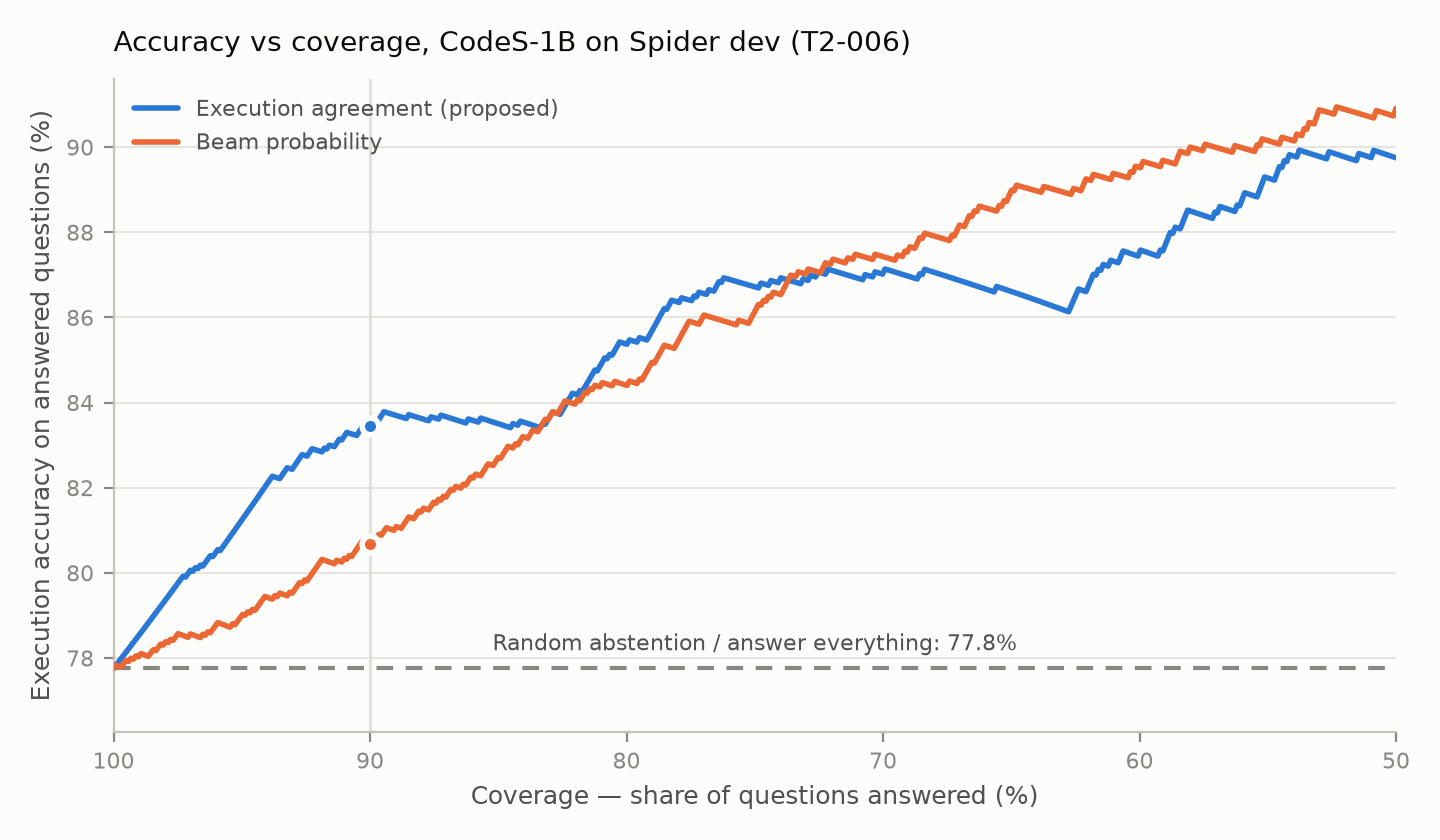
\includegraphics[width=\columnwidth]{figures/accuracy_coverage_T2-006.png}
\caption{Accuracy on answered questions against coverage (CodeS-1B, Spider dev).}
\label{fig:curve}
\end{figure}

\textbf{Why it works, and where it does not.} Accuracy rises steadily with the number of candidates that agree (Table~\ref{tab:levels}): when the answer's result is produced by no other candidate it is right 56.8\% of the time, and when all four agree 88.4\%. When the returned query does not run at all the answer is never right. Agreement is not calibrated at the top, however: 11.7\% of answers on which all four candidates agree are still wrong, because beam candidates share the model's blind spots. Over the whole curve beam probability ranks answers slightly better (area under the risk--coverage curve 0.0905 against 0.1025 for agreement; random 0.2224, perfect ranking 0.0269); agreement is ahead from full coverage down to about 74\% coverage, the region where the operating point lies. Agreement takes only five values, so intermediate coverages rely on the beam-probability tie-breaker.

\begin{table}[t]
\centering
\caption{Accuracy by number of candidates (of 4) that agree with the returned answer (CodeS-1B, run T2-006).}
\label{tab:levels}
\small
\begin{tabular}{@{}lrrrrr@{}}
\toprule
Agreeing candidates & 0 & 1 & 2 & 3 & 4 \\
\midrule
Questions & 28 & 132 & 225 & 237 & 412 \\
Accuracy & 0.0\% & 56.8\% & 75.6\% & 82.3\% & 88.4\% \\
\bottomrule
\end{tabular}
\end{table}

\section{Are the Candidates Really Different?}
\label{sec:diversity}
A natural objection is that beam search often returns the same query several times, in which case agreement among the candidates would mean little, and a related question is why the number of candidates is four. This was also raised at a review of this work, so we measured it. We re-executed every saved candidate of run T2-006.

\textbf{Duplicates.} Here two candidates are the same query if they differ only in spacing or capitals (so alias renamings count as different, which makes this a lower bound on duplication). The four beams are four different queries for only 577 of 1,034 questions (55.8\%); 42 questions have one distinct query, 190 two and 225 three. For CodeS-3B the counts are 57, 234, 249 and 494.

\textbf{Agreement over different queries.} We recomputed agreement (``v2'') counting each different query once and comparing results up to row and column order, which also corrects 68 questions where only the column order hid agreement. Over different queries, accuracy rises with the number that agree: 0 agree: 0.0\% (28 questions); 1: 71.7\% (244); 2: 78.7\% (367); 3: 83.1\% (207); 4: 89.4\% (188). Table~\ref{tab:signals} shows that the abstention gain is unchanged in kind: $+5.14$ points as a share and $+5.66$ as a count, against $+5.46$ for the evaluated rule. The conclusion does not depend on duplicates.

\begin{table*}[t]
\centering
\caption{Abstention signals compared (mean of ten calibration/test splits; gain over random abstention at the same coverage; paired $t$-test $p$; Wilcoxon $p=9.8\times10^{-4}$ in every row). AURC: area under the risk--coverage curve, lower is better. Beam probability and the count variant are not meaningful for sampled candidates (repeats are signal there) and are omitted.}
\label{tab:signals}
\small
\begin{tabular}{@{}llrrrrr@{}}
\toprule
Run (model, candidates) & Signal & Coverage & Acc.\ answered & Gain & $p$ ($t$-test) & AURC \\
\midrule
\multirow{4}{*}{T2-006 (CodeS-1B, 4 beams)} & agreement (evaluated) & 90.5\% & 83.3\% & $+5.46$ & $7.7\times10^{-10}$ & 0.103 \\
 & agreement over different queries (share) & 90.6\% & 82.9\% & $+5.14$ & $1.7\times10^{-9}$ & 0.101 \\
 & agreement over different queries (count) & 90.0\% & 83.5\% & $+5.66$ & $4\times10^{-11}$ & 0.122 \\
 & beam probability & 89.7\% & 80.9\% & $+3.08$ & $9.3\times10^{-7}$ & 0.091 \\
\midrule
\multirow{4}{*}{T2-004 (CodeS-3B, 4 beams)} & agreement (evaluated) & 89.7\% & 85.2\% & $+3.18$ & $2.9\times10^{-6}$ & 0.078 \\
 & agreement over different queries (share) & 89.1\% & 85.9\% & $+3.88$ & $3.6\times10^{-7}$ & 0.072 \\
 & agreement over different queries (count) & 89.4\% & 85.9\% & $+3.95$ & $1\times10^{-7}$ & 0.091 \\
 & beam probability & 88.5\% & 85.4\% & $+3.44$ & $2.9\times10^{-7}$ & 0.065 \\
\midrule
\multirow{2}{*}{SM-008 (CodeS-1B, 8 samples)} & agreement (evaluated) & 90.0\% & 82.5\% & $+5.57$ & $1.7\times10^{-7}$ & 0.109 \\
 & agreement over different queries (share) & 89.5\% & 83.1\% & $+6.19$ & $1.5\times10^{-8}$ & 0.102 \\
\bottomrule
\end{tabular}
\end{table*}

\textbf{Another model.} For CodeS-3B agreement gives $+3.18$ points ($89.7\%$ coverage, $85.2\%$ accuracy on answered) and, over different queries, $+3.88$. Abstention helps the larger and the smaller model, by less for the larger one, which is already right more often. For CodeS-3B, however, beam probability is as good a signal as agreement ($+3.44$ points), so the advantage of agreement over beam probability seen for CodeS-1B does not carry over (Fig.~\ref{fig:curves2}, left).

\textbf{Sampled candidates.} We also drew eight candidates by sampling (temperature 0.8) instead of beams (run SM-008). Plain accuracy is 77.08\% (beams: 77.76\%); a correct query is among the eight for 881 questions (85.2\%) against 859 (83.1\%) among four beams. Majority vote over the eight reaches 77.66\%, whereas majority vote over four beams was worse than the first-executable rule (75.73\% against 77.76\%). Agreement abstention holds (Table~\ref{tab:signals}, Fig.~\ref{fig:curves2}, right), and the 491 questions on which all eight agree are correct 93.5\% of the time.

\begin{figure*}[t]
\centering
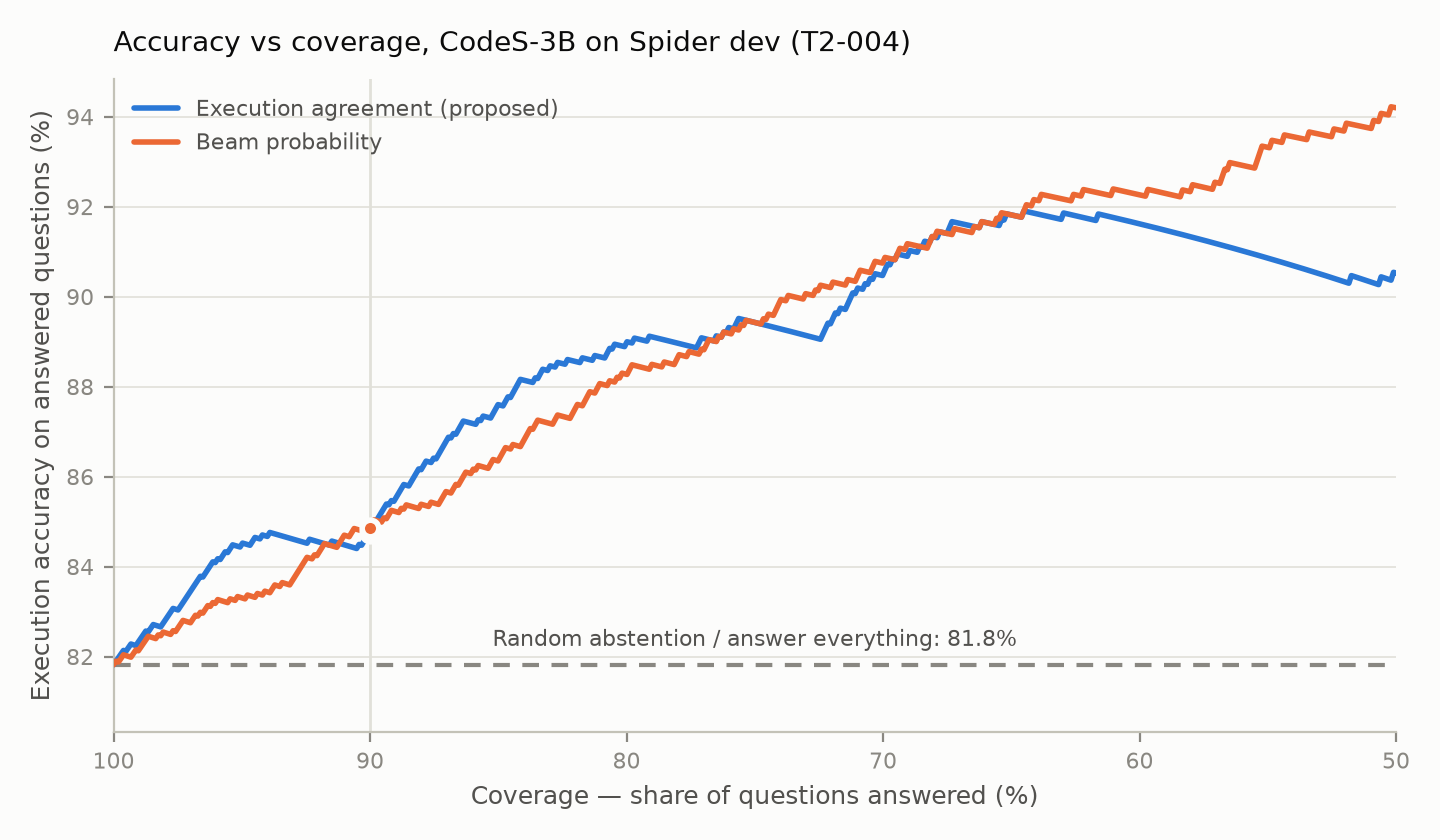
\includegraphics[width=0.43\textwidth]{figures/accuracy_coverage_T2-004.png}\hspace{0.04\textwidth}
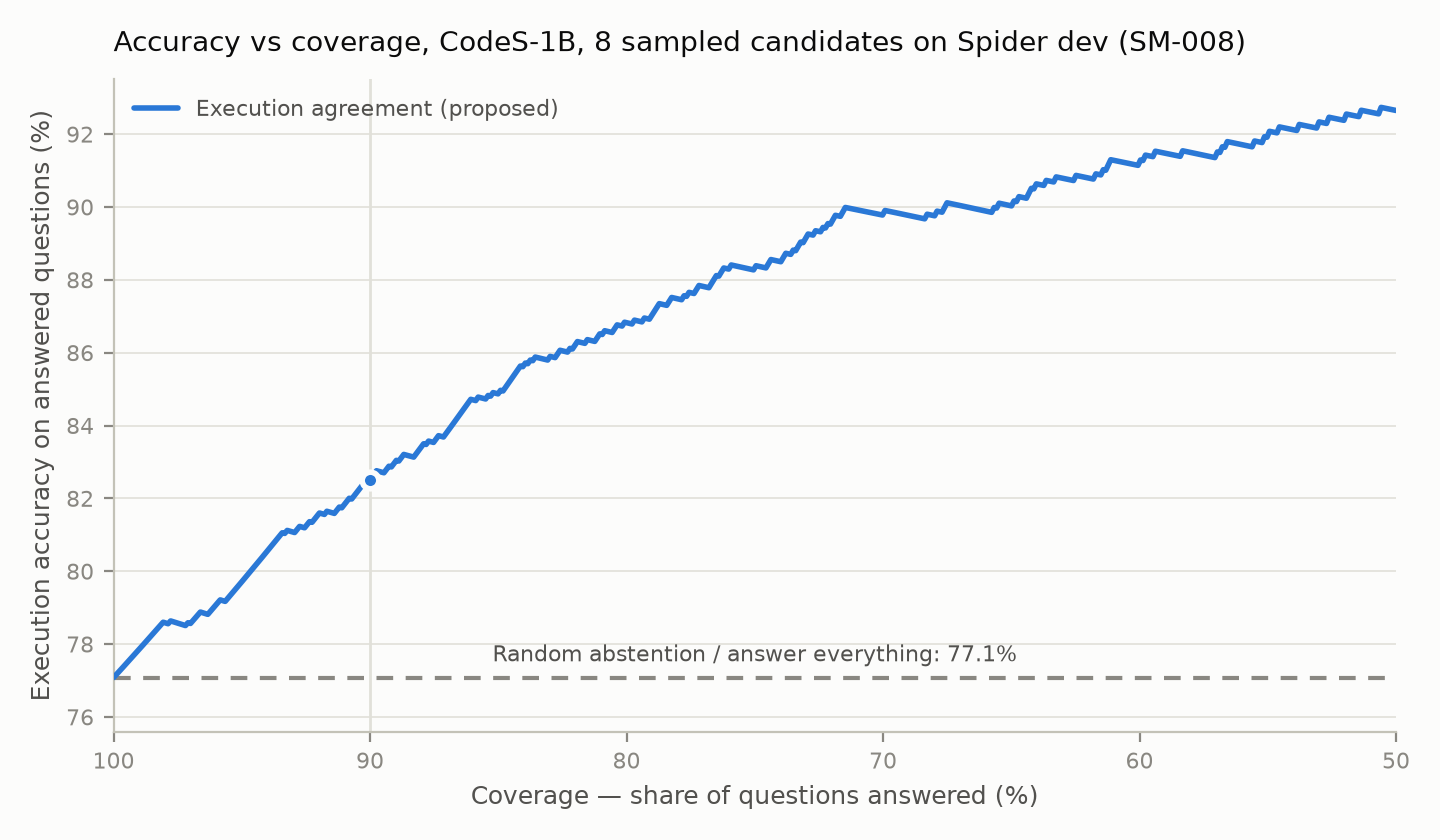
\includegraphics[width=0.43\textwidth]{figures/accuracy_coverage_SM-008.png}
\caption{Accuracy against coverage for CodeS-3B with four beams (left) and CodeS-1B with eight sampled candidates (right). Beam probability is not drawn for sampled candidates.}
\label{fig:curves2}
\end{figure*}

\textbf{Why four?} Four is what CodeS's inference code returns and what our threshold was calibrated on. The application now lets the user choose 2--12 candidates, over-generating beams (or sampling at rising temperature until the queries differ) so that candidates are different queries wherever the model has more than one way to answer. This was done after the evaluation: the measured accuracy and threshold are for four beams, and other counts are uncalibrated. A run with eight beams printed 78.8\% accuracy before it failed while saving its results; it is being re-run, and no further number from it is reported (TBD).

\section{Beyond Spider}
\label{sec:beyond}
\textbf{Rewritten questions.} Spider questions often name the columns. On the 508 development questions that Spider-Realistic \cite{deng2020structuregrounded} rewrites without column names, the pipeline (run on an Apple M4) reaches 69.5\% (353/508) against the paper's 70.9\% ($-1.4$ points). On the original wording of the same 508 questions it reaches 72.8\% (370/508), so the wording costs 3.3 points (bootstrap 95\% CI $[0.8, 5.9]$; 31 questions right only in the original wording, 14 only in the realistic one; exact McNemar $p=0.016$). On the same 508 questions the M4 run chose the same SQL as the T4 run on 485, and accuracy was 72.8\% against 73.2\%. Agreement stays informative (Table~\ref{tab:realistic}): accuracy is 86.9\% when all four candidates agree and 47.1\% when one does. A run on BIRD Mini-Dev \cite{li2023can} was stopped after 18 of 500 questions and is not reported (TBD).

\begin{table}[t]
\centering
\caption{Original and Spider-Realistic wording of the same 508 questions (CodeS-1B).}
\label{tab:realistic}
\small\setlength{\tabcolsep}{3pt}
\begin{tabular}{@{}lrr@{}}
\toprule
 & Original & Realistic \\
\midrule
EX, answering everything & 72.8\% (370) & 69.5\% (353) \\
Balanced: questions answered & 88.6\% & 86.2\% \\
Balanced: accuracy on answered & 79.3\% & 76.7\% \\
Wrong answers, all $\to$ balanced & 138 $\to$ 93 & 155 $\to$ 102 \\
\bottomrule
\end{tabular}
\end{table}

\textbf{A live database.} CodeS writes SQLite. For a server database we translate each query with sqlglot, accept only one read-only statement, and run it in a read-only transaction with a timeout and a row limit; the schema and a value index are read once at connection time. We copied the 20 Spider development databases into PostgreSQL 14 and ran every gold query and every saved prediction on both engines (Table~\ref{tab:pg}). The final rewrites (string literals, case-insensitive \texttt{LIKE}, aggregate grouping) bring agreement between the engines from about two thirds to about 94\%; most remaining mismatches are \texttt{ORDER BY}\ldots\texttt{LIMIT} queries with tied rows, which legitimately differ between engines. End-to-end accuracy and calibration on PostgreSQL, and MySQL, are not measured (TBD); a qualitative run of twelve questions on one database matched the gold answer ten times.

\begin{table}[t]
\centering
\caption{Queries returning the same rows on PostgreSQL as on SQLite.}
\label{tab:pg}
\small\setlength{\tabcolsep}{3pt}
\begin{tabular}{@{}lrr@{}}
\toprule
 & Gold queries & Model predictions \\
\midrule
Plain translation & 67.0\% & 71.1\% \\
\textbf{Final rewrites} & \textbf{94.4\% (976/1034)} & \textbf{93.7\% (943/1006)} \\
\quad different rows / errors & 41 / 17 & 49 / 14 \\
\bottomrule
\end{tabular}
\end{table}

\section{The Application}
\label{sec:app}
The system ships as a desktop application (macOS; a Windows build is configured but untested) that runs the same evaluated code as the experiments (Fig.~\ref{fig:app}). Every answer shows how many of the candidate queries agree; the ``all queries'' view runs and displays every candidate with its own result, marks copies, and shows the repair of a failed query. The user chooses how strict the system is (answer everything, balanced, strict, very strict), with the measured coverage and accuracy of Table~\ref{tab:abstain} shown next to each choice, and when the system abstains it lists the competing readings. Databases can be the built-in samples, a SQLite file or a live PostgreSQL or MySQL server; a saved server connection keeps its password in the operating system's keychain, never in a file. The model is the evaluated CodeS-1B by default, and local CodeS variants, Ollama models and hosted services can be chosen; only CodeS-1B with four beams has measured accuracy, and a hosted service receives the schema, a few example values and the question (result rows only if the user opts in to sharing earlier rows for follow-ups). Follow-up questions use the earlier questions of a chat as context for chat models only, because CodeS was trained on single questions. The core package has 55 model-free tests and is released under the Apache-2.0 licence.

\begin{figure*}[t]
\centering
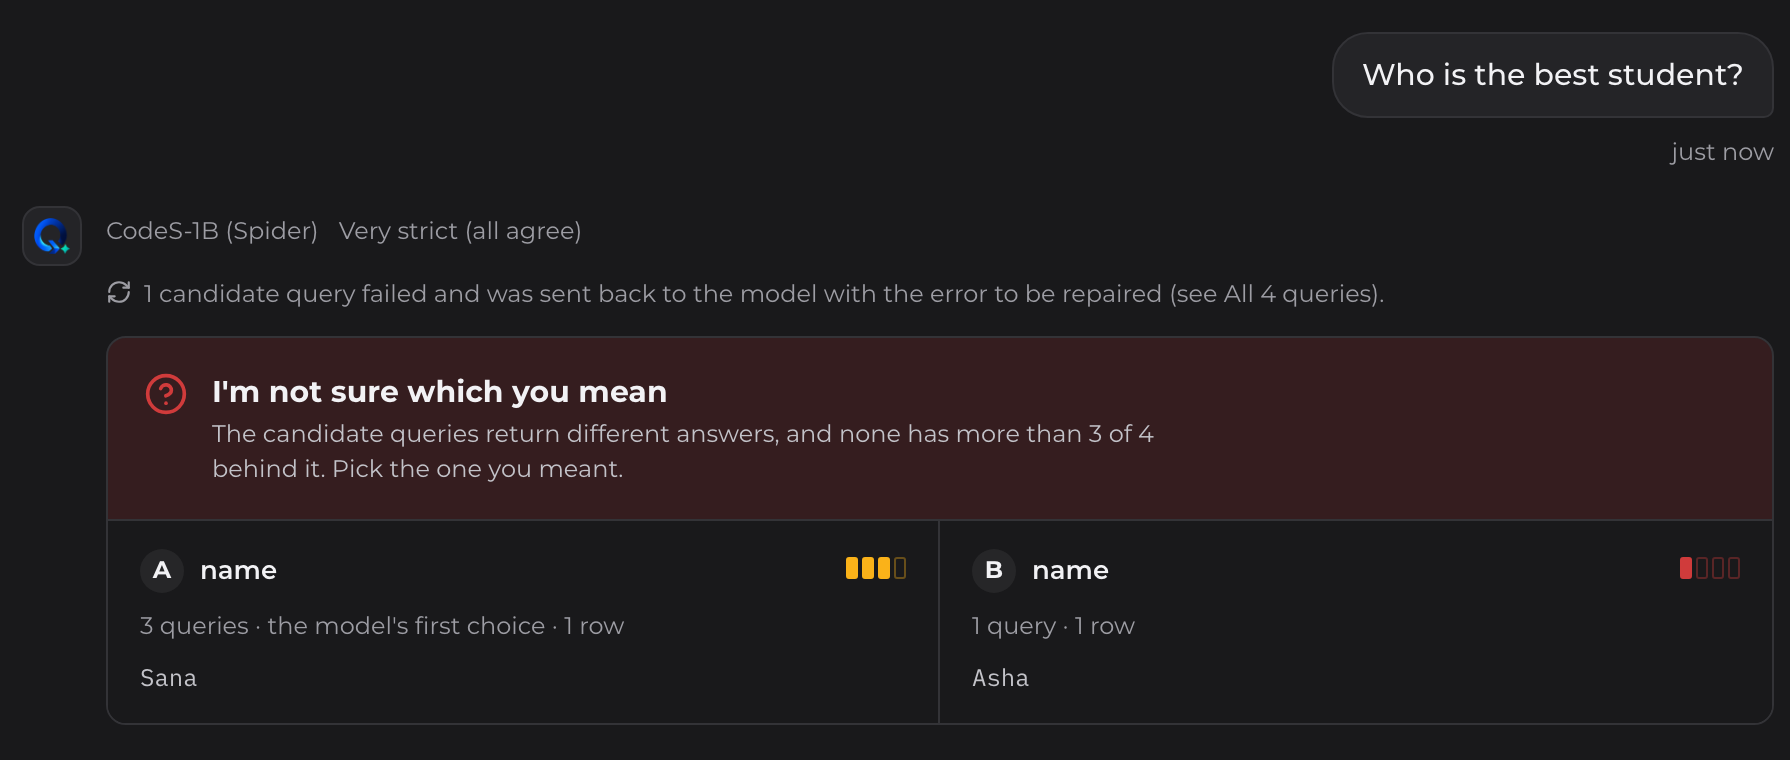
\includegraphics[width=0.78\textwidth]{figures/app_screens.png}
\caption{The application when it is not sure (very strict setting). Three of the four candidate queries return one result (reading A) and one returns another (reading B); that is not enough agreement, so the system lists the readings with their support instead of answering. One candidate failed and was repaired, as the note above the card says.}
\label{fig:app}
\end{figure*}

\section{Discussion and Threats to Validity}
\textbf{What the results say.} The model's own candidates carry usable information about its reliability: declining the 9.6\% least-agreed questions removes 74 wrong answers at the price of 25 correct ones (3.1\% of the 804 the model gets right), and the three strictness settings give the user a dial between coverage and accuracy. The gain holds when duplicates are removed, for a second model size and for sampled candidates, so it is not an artefact of repeated beams. It is also modest and bounded: unanimous candidates are still wrong 11.7\% of the time, and for the 3B model a cheaper signal, beam probability, is as good.

\textbf{Internal validity.} The deployed threshold was chosen on the same development set it is reported on; the split protocol and bootstrap guard against over-fitting to a particular half but not against the set itself. Each configuration was run once with seed 42; beam search is deterministic (a repeat of one run was identical), but the sampled run has not been repeated with other seeds. The Colab and M4 runs agree on 485 of 508 selected queries, so hardware has a small effect. \textbf{Construct validity.} Correctness is Spider's execution match on one database instance per schema; a stricter oracle such as test-suite accuracy can change the labels and so the measured risk \cite{liu2026certified}, and we have not computed it. \textbf{External validity.} Spider's databases are small and clean; the Spider-Realistic gap of 3.3 points shows sensitivity to wording, and BIRD, the larger real-world benchmark, is TBD, so we make no claim about enterprise databases.

\textbf{Limitations.} (1) One benchmark and, for the main result, one model. (2) The ten splits reuse the same 1,034 questions. (3) The ablation differences are small and untested for significance. (4) Test-suite accuracy, BIRD, MySQL and end-to-end PostgreSQL accuracy are TBD, and the larger CodeS models were not run. (5) Candidate counts other than four, and models other than CodeS-1B, are uncalibrated. \textbf{Responsible use.} The default setup runs on the user's machine with open weights and read-only database access, so no schema or data leave it; choosing a hosted model sends the schema to its provider, and the application says so.

\section{Conclusion and Future Work}
An open 1B-parameter text-to-SQL model can be reproduced to within 0.2 points of its published accuracy and made to decline the questions it is likely to get wrong: at 90.4\% coverage it is right 83.3\% of the time instead of 77.8\%, with a third fewer wrong answers, using only the candidates it already generates and no retraining. The result survives duplicated candidates, a larger model and sampled candidates, and the system works on rewritten questions and a live server database. Next steps are the results marked TBD (test-suite accuracy, BIRD, the eight-beam run, MySQL and end-to-end PostgreSQL accuracy), calibrating the threshold for other candidate counts, per-database adaptation, and role-based access when connected to a company database.

\section*{Acknowledgment}
The authors thank M Parameswar for supervision, and the Department of Computer Science \& Information Technology, KL University, for the project framework.

\bibliographystyle{IEEEtran}
\bibliography{references}

\end{document}
